\section{Binary Trees}

While a tree ADT can have any number of branches theoretically, often we
limit the number of branches. A binary tree (one with nodes that can
have at most two branches ) is a very common ADT. 

\subsection {C Structure for Binary Tree ADT}

As with any ADT, the Binary tree needs a structure to hold the pointers
to its connected nodes and to hold a pointer to the data. A binary tree
node is usually labeled with pointers called `left' and `right' to
denote the child nodes.

\begin{lstlisting}
struct BinTreeNode
{
	void * data
	struct BinTreeNode * left
	struct BinTreeNode * right
	Tree * myTree;  //not required, but  useful for getting the function pointers
};

struct BinTree
{
	int compare function
	void destroy function
	Struct BinTreeNode * root;
};

typedef Struct BinTree Tree;
\end{lstlisting}

Because the Binary Tree ADT stores \emph{void * } data,  the user of the tree ADT must supply a function pointer for
the destruction of the data and clean up of memory as well as for comparing data elements to determine the position of the data in the tree.

  The Tree ADT
must guarantee that all nodes that are removed, either individually
or when the tree is destroyed, will be properly removed from memory
using the supplied function. 

Also, because data in a binary tree is kept
in sorted order, the user of the ADT must supply a function pointer to a
compare operation that can compare the values of two data items. (If you
are fuzzy about function pointers, go back to the function pointer
review).

Binary tree operations can be divided into two sets. The first set are
sometimes called wrapper operations  These are the operations that the
user of the ADT will call.  Wrapper functions typically take the Tree Struct as a parameter, possibly along with other paramters.

The second set of operations are the helper
operations. These are the operations that actually do the work of
setting up, manipulating, and keeping track of the tree.  The helper operations typically take the root node of the tree as a parameter ( the \textbf{root} member variable of the Tree struct) along with other paramters.  Often helper operations for trees are recursive.
Below you can find a list of some common wrapper and helper operations on binary trees.

\begin{lstlisting}

//ADT Wrapper Operations

createBinaryTree( compare function pointer, destroy function pointer):BinTree
destroyBinaryTree(BinTree *): void *
addToTree (void * data)
removeFromTree(void * data): Boolean
findInTree(void * data):void *

//Helper Operations

TreeNode * insert(TreeNode * root, TreeDataType data);
TreeNode * delete(TreeNode * root, TreeDataType data);
bool isEmpty(TreeNode * root);
bool hasTwoChildren(TreeNode * root);
int compare (TreeDataType data1, TreeDataType data2);
TreeNode * findMinimum(TreeNode * root);
void printInOrder(TreeNode * root);
\end{lstlisting}

In addition to wrappers and helpers, most tree ADTs provide operations
that will traverse the tree and do something during the traversal. The
elegant way to provide node-processing functionality is to provide
traversal operations that accept a function pointer. The function is
executed once for every node in the tree.

Lets start our exploration of binary trees by looking at the helper
functions starting with insertion. We'll ignore the data types and
function pointers for now, but will return to them towards the end of
this chapter.

\subsection{Recursive Helper Functions}
\subsubsection{Insertion}

Insertion into a tree has three possible cases:

\begin{enumerate}
\item
  The tree has no nodes, and the value will be inserted as the root node
\item
  The value to be inserted is larger than the value at the root, and
  will be inserted in the right subtree of the root node.
\item
  The value to be inserted is less than the value of the root, and will
  be inserted into the left subtree of the root node.
\end{enumerate}

Cases 2 and 3 result in a recursive call to the insertion operation.

\begin{lstlisting}
insert(TreeNode * root, TreeDataType data, funcPointer to compare operation): TreeNode *

if (the root node is empty)
{
	allocate memory for a TreeNode and assign it to temp
	temp-\textgreater{} data = data
	temp -\textgreater{} left = NULL;
	temp -\textgreater{} right = NULL;
	return temp;
}
if(compareFunction(root-\textgreater{}data, data) shows root data is smaller)
{
	/*recursively call insert on right subtree*/
	root-\textgreater{}right = insert(root-\textgreater{}right,data, comparePointer)
}
else if(compareFunction(root-\textgreater{}data, data) shows root data is larger)
{
	/*recursively call insert on left subtree */
	root-\textgreater{}left =insert(root-\textgreater{}left,data,comparePointer);
}
/* Else there is nothing to do as the data is already in the tree. */
return root;
}
\end{lstlisting}


Because a binary tree is stored in sorted order, insertions have to be
done by comparing the data to be inserted to the data stored at the
current node. Insertions are always done at a leaf node. By supplying a
function pointer for the comparison operator, a tree ADT can
successfully insert any type of data.

Here is a visual look at the insert operation.

Suppose we wanted to insert 17 into the tree shown.

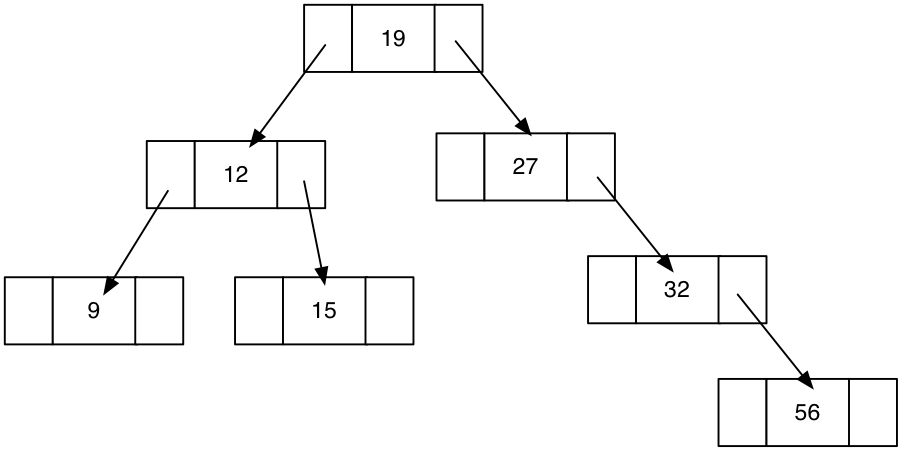
\includegraphics[width=6.00000in]{pictures/bintree1.png}

We first compare 17 to the value at the root node (19). Since 17 is
less than 19, and in this binary tree we are storing the smallest values in the left subtree,  we recursively call the insert procedure on the left
subtree of 19.

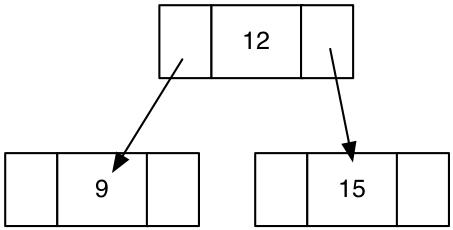
\includegraphics[width=3.01389in]{pictures/bintree2.png}

We compare 17 to the root node of the subtree. 17 is greater than 12, so
we recursively call the insert procedure the right subtree of 17- which is the node containing 15.


17 is larger than 15, so we recursively call the insert procedure on the
right subtree of 15. That subtree is a NULL tree, which activates the
base case of the recursive algorithm.

A node is made for 17, the pointer to it is returned as the recursion
unwinds.

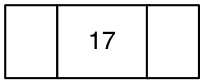
\includegraphics[width=1.34722in]{pictures/bintree3.png}

On the way back up, the tree reassembles each level.

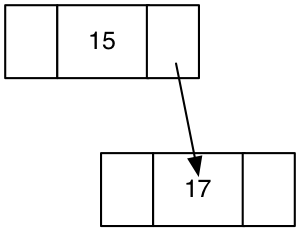
\includegraphics[width=1.98611in]{pictures/bintree4.png}

Then

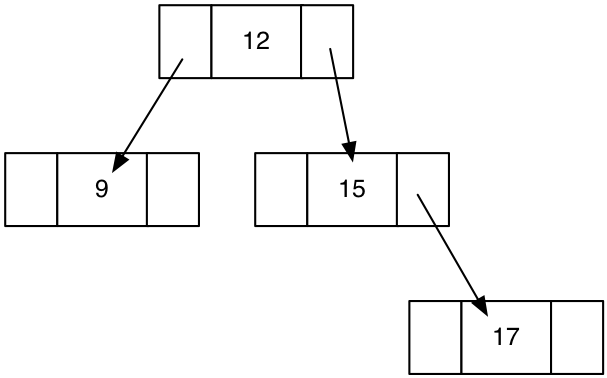
\includegraphics[width=3.65278in]{pictures/bintree5.png}

and finally back to the entire tree.

\subsubsection{Deletion}

Deletion from a binary tree is a bit trickier because you have to be
careful to keep the tree in the proper order.

There are three cases to consider when deleting a node from a binary
tree:

\begin{enumerate}
\def\labelenumi{\arabic{enumi})}
\item
  the node has no children
\item
  the node has only one child (left or right branch)
\item
  the node has two children
\end{enumerate}


The first case is easy. If the node to be deleted has no children (i.e.
it is a leaf node) it can be deleted and the appropriate branch of its
parent set to NULL.

In the second case, If the node to be deleted has a right branch child,
then the deleted node's parent can be set to point at the child and the
tree will remain in the correct order.

Suppose we needed to delete 32 from the subtree below. We could simply
remove 32 and set 27 to point at 56 and the properties of the binary
tree would not have changed.

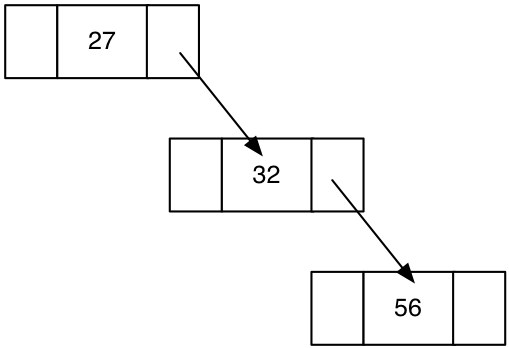
\includegraphics[width=3.38889in]{pictures/bintree6.png}

If a node has a left child only, the same process can be used to remove
the node. Attach the nodes left child to the node's parent and the tree
structure will still be valid.

The more complicated case arises when the node to be deleted has two
children.

Suppose that we want to delete node 12 from this tree. We can't simply
remove 12 and put either one of its children in its place, because we
would lose part of a subtree. If 15 replaced 12, there would be no place
to reattach 9 and a similar problem exists if 9 were used to replace 12.

%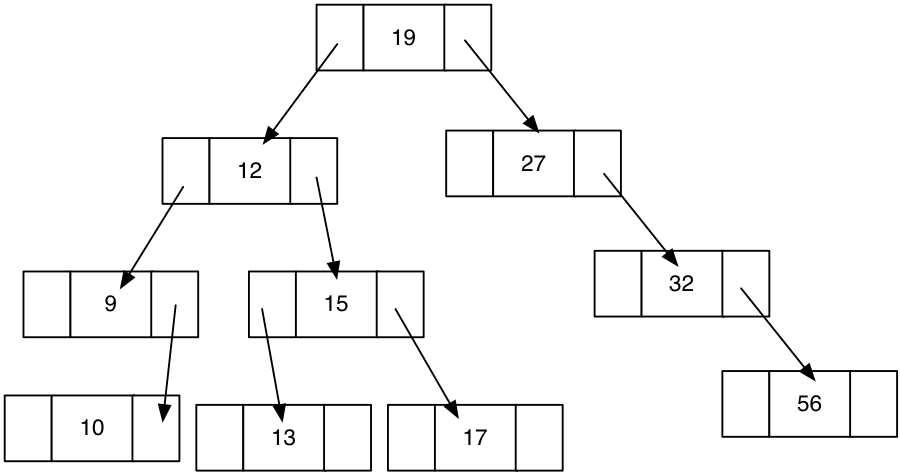
\includegraphics{pictures/bintree7.png}

The problem is solved by remembering that the right subtree always
contains values that are larger than the node, and the left subtree
contains values that are greater. So, for any node, the smallest value
in the left subtree will be a node that has a value slightly larger
than the node being removed, but smaller than all the other nodes in the
subtree. That node will also be a leaf node in the tree.

The algorithm is this:

\begin{itemize}
\item
  find the minimum value in the right subtree of the node to be deleted
\item
  copy that value into the node to be deleted (temporarily making a
  duplicate node)
\item
  recursively call delete on the right subtree -- for the value we just
  copied in. This will activate the base case of the node having no
  children and will remove the node
\end{itemize}

In the case of the previous example, we would copy the value 13 into the
node that presently holds 12, and then call delete (13) on the subtree
rooted at 15. The node at 13 will be removed and the tree will look like
this:

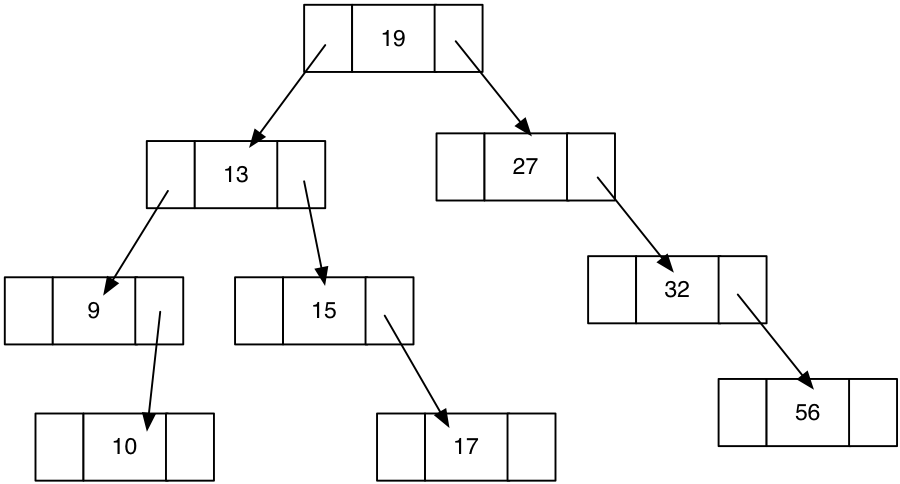
\includegraphics[width=6.00000in]{pictures/bintree8.png}

\begin{lstlisting}
TreeNode * delete(TreeNode * root, TreeDataType data, compareFP,destroyNodeFP):TreeNode

TreeNode * temp;
TreeDataType removedData;

if the root is empty
	we have a problem and should clean up and exit gracefully
else if (compareFP(root-\textgreater{}data, data) shows that the root data is larger)
{
	root-\textgreater{}left = delete(root-\textgreater{}left, data, compareFP, destroyNodeFP);
}
else if (compareFP(root-\textgreater{}data, data) shows that the searched for data is larger)
{
root-\textgreater{}right = delete(root-\textgreater{}right,data,compareFP, destroyNodeFP);
}
else /*the comparison is equal and we can delete the node we've found */
{
	if (the root node has two children) /*replace this node with the smallest element in right subtree */
	{
		temp = findMinimum(root-\textgreater{}right)
		removedData = root-\textgreater{}data
		destroyFP(root-\textgreater{}data) /*now call destroy function on that data */
		root-\textgreater{}data = temp-\textgreater{}data
		root-\textgreater{}right = delete(root-\textgreater{}right,
		temp-\textgreater{}data,compareFP, destroyFP)
	}

	else  /*this node has zero or one child*/
	{
		temp = root;
		if (root-\textgreater{}left == NULL) /* we have no left child */
		{
			root = root-\textgreater{}right;
		}

		else if (root-\textgreater{}right == NULL) /*we have no right child */
		{
			root = root-\textgreater{}left;

		}
	}
	/*either we've rejoined the subtree, or we're about to delete a leaf node*/

	destroyFP(temp-\textgreater{}data);/*call destroy function on temp-\textgreater{}data */
	free(temp);

}
\end{lstlisting}
\subsection{Wrapper functions}

The wrapper functions for a Tree ADT provide the interface that the user
of the ADT interacts with.
The wrapper functions are not recursive rather, they call the recursive
functions when appropriate.

\begin{itemize}
\item {createBinaryTree( compareFP, destroyNodeFP)): Tree *

createTree is used to initialize a tree and to set up the function
pointers for the data type that the tree will be storing. When function
pointers are used, and data is cast to a void pointer, the same compiled
tree library can be used to hold any kind of data.
}
\item {destroyBinTree(Tree * toDie)

destroyBinTree is called when the tree must be released. The destroy
tree function will recursively destroy all the tree nodes AND all of the
data elements (using the supplied function pointer).
}

\item {addToTree(Tree, void * )

addToTree inserts a value into the tree by calling the recursive insert function.
}

\item {removeFromTree(Tree*, void *)

removeFromTree searches for the data provided in the parameter and, if found, removes that data from the tree.  Remove from tree should also free the memory allocated for the node.  It is a design choice as to whether removeFromTree also frees the memory for the data.

}

\item {findInTree(Tree *, void *):Boolean 

findInTree returns true(1) if the data is found, false(0) if not.
}

\end{itemize}

The wrapper functions are usually not complicated and mostly call the recursive helper function for the
appropriate operation, passing in the function pointers and parameters to the operation as necessary. See the given code
for addToTree for an example.

\begin{lstlisting}
void addToTree (Tree* theTree, void * data)
{
	theTree-\textgreater{}root = insert(theTree-\textgreater{}root, data,theTree-\textgreater{}compare);
}

\end{lstlisting}


\subsubsection{Traversals}

Another common set of functions for trees are traversal algorithms.  A traversal algorithm can also be used to create an \textbf{iterator} for a tree. Traversal algorithms were introduced in the introductory section on single-rooted trees.  In addition to the  in-order and pre-order traversals explored in that section,  a tree traversal can be written to be in post-order (the root is processed after the subtrees- left subtree, right subtree, root)  or in level-order where the root is processed,  then all of the root's immediate children,   then all of the root's grandchildren,  then all of the root's great grand children, etc.  A level-order traversal is also known as a breadth-first traversal.

A recursive algorithm for a level-order traversal of a tree is shown below.   

\begin{lstlisting}
for ( the height of the tree)
{
    processLevel(TreeNode * root, height)
}

void processLevel( TreeNode * currentNode, int level )
{
    if ( currentNode  is NULL)
        return;
    if (level == 1)
        process  currentNode->data //processing could be printing or something else
    else if (level > 1)
    {
        processLevel(currentNode->left, level-1)
        processLevel(currentNode->right, level-1)
    }
\end{lstlisting}



Often a traversal function will take a function pointer as an argument
and will apply that function to the data in each node of the tree. For
example, you could write a function that printed a node value, and then
combine that function with a traversal function to print the tree in a
variety of orders. 

The print function is data dependent,but the traversal function is not.  
For example, a function to print  integer data might look like this:

\begin{lstlisting}
void printIntNode(void * data)
{
	printf("\%d ", data);
}

\end{lstlisting}

where a function to print values from a tree that was storing strings
might look like this

\begin{lstlisting}
void printStringNode(void * data)
{
	printf("\%s ", data);

}
\end{lstlisting}

A traversal algorithm could be called, sending it the print function,
and any type of data could be successfully printed. For example.
\begin{lstlisting}
printInOrder(myTree-\textgreater root, \&printIntNode);

//or

printInOrder(myTree-\textgreater root, \&printStringNode);
\end{lstlisting}

The key to remember that the user of
the ADT is the one who defines the data stored by the ADT and the
operations to compare, destroy, and manipulate that data. The tree ADT
simply stores the data and performs the requested operations when given
pointers to those operations.


\section{Types of Binary Trees}

A binary tree is \textbf{full} if every node in the tree has zero or two children.     A full binary tree has the property where the number of leaf nodes (L) is equal to the number of internal nodes (I) + 1.    If you are curious about the proof of this propertly see
 \url{http://www.geeksforgeeks.org/handshaking-lemma-and-interesting-tree-properties/}
  \begin{figure}[H]
\centering
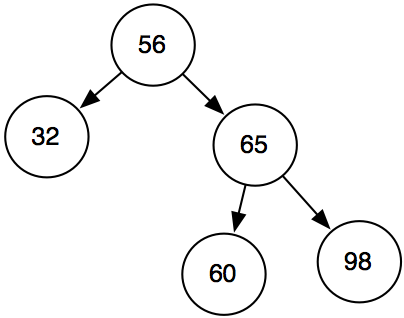
\includegraphics{pictures/fullTree.png}
\label{fig:fullTree}
\caption{A full binary tree}
\end{figure}

A binary tree is \textbf{complete} if all the levels of the tree are full excepting possibly the last level.   The last level must have all the nodes as far to the left hand side of the tree as possible.    A complete binary tree is used in the implementation of a \textbf{heap}.

  \begin{figure}[H]
\centering
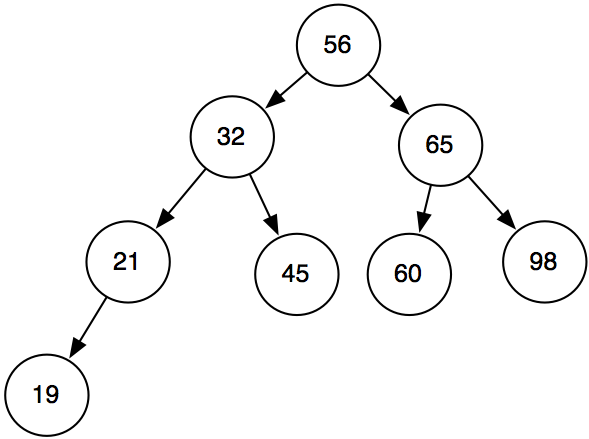
\includegraphics{pictures/completeTree.png}
\label{fig:fullTree}
\caption{A complete binary tree.  All of the levels in the tree have two child nodes except for the last level.  The child nodes in the 
last level are as far left as possible.}
\end{figure}

A \textbf{perfect} Binary tree is one in which all internal nodes have two children.   The leaf nodes of a perfect binary tree are all at the same level.
The number of nodes in a perfect binary tree is $2^h-1$ where h is the height of the binary tree.  

  \begin{figure}[H]
\centering
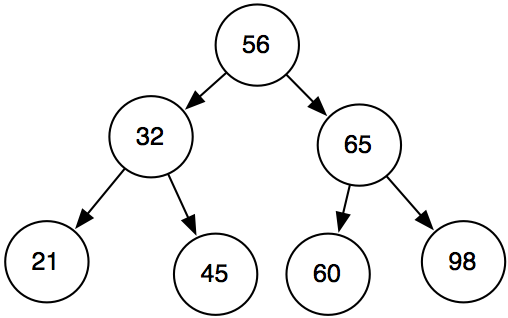
\includegraphics{pictures/perfectTree.png}
\label{fig:fullTree}
\caption{A full binary tree}
\end{figure}

 

\section{Extending Activities}

\begin{itemize}


	\item {The order that nodes are inserted into a tree can greatly affect the
	structure of the tree. Draw the binary tree that is constructed by adding the
	seven names in the following order:
	
	\begin{itemize}
	\item
	  Sleepy
	\item
	  Bashful
	\item
	  Doc
	\item
	  Dopey
	\item
	  Sneezy
	\item
	  Happy
	\item
	  Grumpy
	\end{itemize}
	}



\item{ Trace the algorithms for level-order traversal using a hand
drawn tree.  What order are the nodes of the tree printed in?  Can you tweak the algorithm to reverse the order?
}
	
	
	
\item{ One of the most frequent uses of a binary tree is as a
search tree. The object is to search through the data to find out if a
particular element is part of the data. Write a recursive find procdure
for a binary tree. Start with the root node of the tree. Your procedure
can be in c or in pseudocode. Be sure to pass in the compare function
pointer.

}



	\item{
	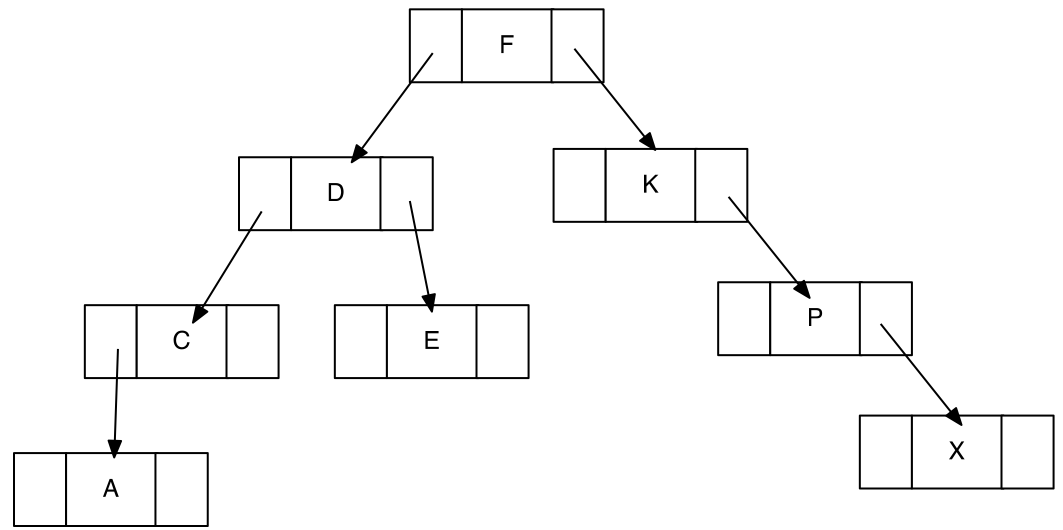
\includegraphics[width=6.00000in]{pictures/image5.png}
	
	Give the in-order traversal of the tree shown above.
	
	Give the pre-order traversal of the tree.
	}

\item Write the pseudocode or c code for a compare operator. A
compare operator must return three distinct values, one for when the
first parameter is larger, one for when the second parameter is larger,
and one for when the two parameters are equal. The convention is to use
1, 0, and -1 for the three values. Zero for equal values, 1 for the
first string being larger, -1 for the second. 


\item The delete operation relies on a recursive function to
find the minimum value in a subtree. The minimum value will always be
the leftmost leaf of the subtree. Write the findMinimum function (in
pseudocode or in C).

\end{itemize}

